Dans cette section, nous présentons l’organisme d’accueil en abordant son histoire, ses valeurs, ainsi que ses partenariats qui contribuent à son succès et à son développement.
\subsection{\texorpdfstring{Aperçu général d'Addinn}{Aperçu général d'Addinn}}
    \begin{minipage}{.6\textwidth}
        \justifying
        Addinn est un cabinet de conseil en transformation digitale spécialisé dans l’accompagnement des entreprises pour définir leur stratégie et mettre en œuvre leurs projets technologiques grâce à un écosystème innovant et complémentaire permet de relever les défis numérique avec succès\cite{Addinn}.\\
    \end{minipage}
    \begin{minipage}{.4\textwidth}
        \vspace{-2.1cm}
        \begin{figure}[H]
            \centering
            
\includegraphics[width=\linewidth]{pages/page-de-garde/img/logo.png}
            \caption{\centering Logo d'\acs{ADDINN}\protect{\cite{Addinn}}}
            \label{fig:logo-ADDINN}
        \end{figure}
    \end{minipage}
\vspace{-0.8cm}
\subsection{Fondements de la Société\cite{apropos}}
    \acs{ADDINN} a pour mission de créer de la valeur à chaque étape de la réflexion à la mise en œuvre et au déploiement des projets \acs{IT}. Son engagement en faveur de l’innovation se reflète dans sa devise "\textbf{ADD} VALUE BY \textbf{INN}OVATION", illustrant sa volonté d’apporter une réelle valeur ajoutée à ses clients. Grâce à son approche novatrice et son expertise, l'entreprise aide à relever les défis avec agilité et efficacité, garantissant ainsi une transformation réussie et durable.\\
    Le tableau~\ref{tab:objectifs} présente les objectifs et les valeurs qui orientent l’approche d’ADDINN:
    \begin{table}[H]
        \centering
        \caption{Synthèse des objectifs stratégiques et des valeurs portées par ADDINN}
        \renewcommand{\arraystretch}{1.5}
        \begin{tabular}{|c|c|}
            \hline
          \textbf{ Objectifs d’ADDINN }  & \textbf{Valeurs d’ADDINN}\\ \hline
            \begin{minipage}{.48\textwidth}
                \vspace{0.15cm}
                 \begin{justify}
                    \begin{itemize}[label=$\bullet$,left=-0.1cm]
                        \item Optimiser les flux de travail afin de les rendre plus rapides et simples.
                        \item Développer des systèmes et des solutions plus efficaces.
                        \item Améliorer l'expérience de clients et accroître l'avantage concurrentiel de l'entité.
                    \end{itemize}
                \end{justify}
                \vspace{0.15cm}
            \end{minipage}
              & 
            \begin{minipage}{.48\textwidth}
                \vspace{0.15cm}
                 \begin{justify}
                    \begin{itemize}[label=$\bullet$,left=-0.1cm]
                        \item \textbf{Innovation}: Pousser plus loin les idées grâce à la recherche et au développement.
                        \item \textbf{Agilité}: Reposer sur la flexibilité et la collaboration comme principes fondamentaux.
                        \item \textbf{Excellence}: Viser la qualité à travers une approche structurée et optimisée.
                    \end{itemize}
                \end{justify}
                \vspace{0.15cm}
            \end{minipage} \\\hline
        \end{tabular}
        \label{tab:objectifs}
    \end{table}
    \vspace{-0.6cm}
\subsection{Fiche de présentation d'ADDINN}
        Le table ~\ref{tab:infoADD} fournit un aperçu détaillé de l'organisme d'accueil.
        \begin{table}[H]
            \caption{\centering Fiche de présentation de la société d'ADDINN \cite{Addinn}\cite{apropos}} 
            \centering
            \renewcommand{\arraystretch}{1.5}
            \begin{tabular}{|p{2.3cm}|p{14cm}|}
                \hline
                    \textbf{Nom} & \textbf{ADDINN}\\
                \hline
                    \textbf{Type} & Société de conseil en transformation digitale\\
                \hline
                    \textbf{Adresses} & 
                        \begin{minipage}{14cm}
                            \begin{justify}
                                \vspace{0.15cm} 
                                \begin{itemize}[left=-0.1cm,label=$\bullet$]
                                    \item \textbf{ADDINN Groupe (France):} 121 Avenue Champs-Elysées Paris 75008.
                                    \item \textbf{ADDINN Tunis:} Immeuble Etraton, Rue Khadija Ben Arfa, Centre Urbain Nord 1082.
                                    \item \textbf{ADDINN Sousse:} Rue Hedi Nouira Akouda Sousse 4022.
                                    \item \textbf{ADDINN Tozeur:} Immeuble Akouri, 2ème étage, rue 2 Mars, Tozeur.
                                    \item \textbf{ADDINN Africa (Congo Brazzaville):} N°3 Allée des Manguiers Beach Centre-ville – Brazzaville.
                                \end{itemize}    
                                \vspace{0.15cm}        
                            \end{justify}
                        \end{minipage}\\
                \hline
                    \textbf{Chiffres Clés} & 
                        \begin{minipage}{14cm}
                            \vspace{0.15cm} 
                            \begin{itemize}[left=-0.1cm,label=$\bullet$]
                                \item Plus de 11 ans d’expérience en consulting IT.  
                                \item Plus de 100 consultants et ingénieurs qualifiés.  
                                \item 90\% des projets gérés en Agile/Scrum.  
                                \item Plus de 40 experts certifiés.  
                            \end{itemize}
                        \end{minipage}\\
                \hline
                    \textbf{Domaines d'expertise} & Conseil en stratégie, conseil en transformation digitale, développement IT et solutions numériques. \\
                \hline 
                    \textbf{Email} & 
                        contact@addinn.com et sales@addinn.com \\
                \hline
                    \textbf{Site web} & \url{https://addinn-group.com/}\\
                \hline
            \end{tabular}
            \label{tab:infoADD}
        \end{table} 
    \vspace{-0.5cm}
    \subsection{Histoire de croissance d’ADDINN et présence internationale\cite{apropos}}
        L’histoire d’ADDINN débute en 2012, avec la rencontre de deux amis ambitieux souhaitant prendre part à la révolution digitale. Plus d’une décennie d’efforts, d’innovations technologiques et de stratégie d’expansion a permis à l’entreprise de franchir ses frontières d’origine.
        \begin{minipage}{.55\textwidth}
            \begin{justify}
                Aujourd’hui, ADDINN Group s’impose comme un acteur clé du marché euro-méditerranéen et africain. Avec son siège social à Paris, le groupe a étendu ses activités en créant 3 filiales en Tunisie, en Mauritanie et au Congo-Brazzaville , comme le montre la figure~\ref{fig:presence_addinn}.
                
                Grâce à des partenariats solides, ADDINN maintient des relations privilégiées avec ses clients au Gabon, en République Démocratique du Congo et en Belgique, consolidant ainsi son expansion à l'international.  
                
                Le tableau~\ref{tab:etapes_addinn} résume les étapes clés de cette croissance.
            \end{justify}
        \end{minipage}
        \hspace{0.1cm}
        \begin{minipage}{.45\textwidth}
            \vspace{-1cm}
            \begin{figure}[H]
                \centering
                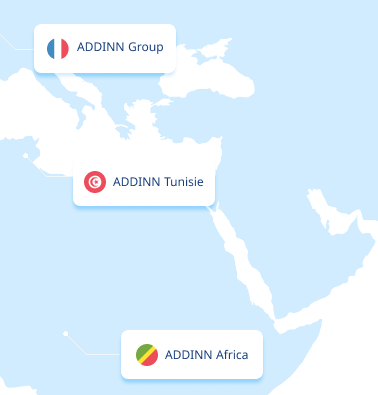
\includegraphics[width=\linewidth]{chapitres/ch1/img/map.PNG}
                \caption{\centering Présence internationale d'ADDINN\cite{apropos}}
                \label{fig:presence_addinn}
            \end{figure}
        \end{minipage}
        \begin{table}[H]
            \centering
            \caption{Étapes Clés d'Évolution d’ADDINN\cite{apropos}}
            \renewcommand{\arraystretch}{1.5}
            \begin{tabular}{|l|p{15cm}|}
                \hline
                \textbf{Année} & \textbf{Événement} \\
                \hline
                \textbf{2015} & Fondation d’ADDINN Group en France, spécialisé dans le conseil en IT. \\
                \hline
                \textbf{2018} & Création de la Digital \& Software Factory, dédiée au développement de solutions numériques sur mesure. \\
                \hline
                \textbf{2022} & Filialisation du groupe avec la création d’ADS Foundry, BeeWay Advisory et Qualifactory, ouvrant une nouvelle phase de développement et de croissance.  \\
                \hline
            \end{tabular}
            \label{tab:etapes_addinn}
        \end{table}
    \vspace{-0.6cm}
\subsection{Secteurs d'expertise et partenaires stratégiques} 
    L'expertise d'ADDINN couvre divers secteurs tels que l'assurance, la banque, le secteur public et le transport, offrant des solutions sur mesure. De plus, l'entreprise collabore avec plusieurs partenaires pour renforcer son offre et sa compétitivité, comme l'illustre la figure \ref{fig:Partenaires}.
    \vspace{-0.3cm}
    \begin{figure}[H]
        \centering
        \renewcommand{\thesubfigure}{}
        \subfloat{
\includegraphics[width=0.16\textwidth]{chapitres/ch1/img/partenaires/a1.png}}
        \subfloat{
\includegraphics[width=0.155\textwidth]{chapitres/ch1/img/partenaires/a2.png}} 
        \subfloat{
\includegraphics[width=0.13\textwidth]{chapitres/ch1/img/partenaires/a9.png}}
        \subfloat{
\includegraphics[width=0.14\textwidth]{chapitres/ch1/img/partenaires/a10.png}}
        \subfloat{
\includegraphics[width=0.15\textwidth]{chapitres/ch1/img/partenaires/a5.png}}
        \subfloat{
\includegraphics[width=0.15\textwidth]{chapitres/ch1/img/partenaires/a11.png}}
        \subfloat{
\includegraphics[width=0.14\textwidth]{chapitres/ch1/img/partenaires/a3.jpg}} \\
        
        \subfloat{
\includegraphics[width=0.17\textwidth]{chapitres/ch1/img/partenaires/a4.png}}
        \subfloat{
\includegraphics[width=0.19\textwidth]{chapitres/ch1/img/partenaires/a12.png}}
        \subfloat{
\includegraphics[width=0.19\textwidth]{chapitres/ch1/img/partenaires/a7.png}}
        \subfloat{
\includegraphics[width=0.14\textwidth]{chapitres/ch1/img/partenaires/a19.png}} 
        \subfloat{
\includegraphics[width=0.15\textwidth]{chapitres/ch1/img/partenaires/a6.png}}
        \subfloat{
\includegraphics[width=0.19\textwidth]{chapitres/ch1/img/partenaires/a17.png}}\\
        
        \subfloat{
\includegraphics[width=0.17\textwidth]{chapitres/ch1/img/partenaires/a13.png}}
        \subfloat{
\includegraphics[width=0.22\textwidth]{chapitres/ch1/img/partenaires/a8.png}}
        \subfloat{
\includegraphics[width=0.17\textwidth]{chapitres/ch1/img/partenaires/a14.png}}
        \subfloat{
\includegraphics[width=0.17\textwidth]{chapitres/ch1/img/partenaires/a15.png}} 
        \subfloat{
\includegraphics[width=0.17\textwidth]{chapitres/ch1/img/partenaires/a16.png}}
        \subfloat{
\includegraphics[width=0.135\textwidth]{chapitres/ch1/img/partenaires/a18.png}}\\
        \caption{Partenaires stratégiques d'ADDINN \cite{Addinn}}
        \label{fig:Partenaires}
    \end{figure}    